\documentclass{beamer}
\usetheme{Madrid}
\usecolortheme{whale}
\usepackage[utf8]{inputenc}
\usepackage[T1]{fontenc}
\usepackage{graphicx}
\usepackage{amsmath}
\usepackage{tikz}
\usetikzlibrary{shapes,arrows,positioning,calc}

\title{Introduction à la GenAI0}
\author{Formation GenAI}
\date{\today}

\begin{document}

\begin{frame}
    \titlepage
\end{frame}

\begin{frame}{Le concept de modèle en IA}
    \begin{itemize}
        \item Un \textbf{modèle} est le composant central de toute IA
        \item C'est un système qui transforme des \textbf{entrées} en \textbf{sorties}
        \item Il capture des \textbf{patterns} à partir de données
    \end{itemize}
    
    \begin{center}
        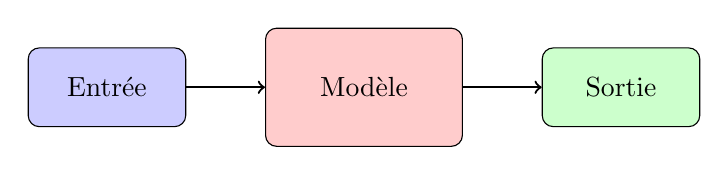
\begin{tikzpicture}
            \node[draw, rounded corners, minimum width=2cm, minimum height=1cm, fill=blue!20] (input) {Entrée};
            \node[draw, rounded corners, minimum width=2.5cm, minimum height=1.5cm, fill=red!20, right=1cm of input] (model) {Modèle};
            \node[draw, rounded corners, minimum width=2cm, minimum height=1cm, fill=green!20, right=1cm of model] (output) {Sortie};
            
            \draw[->, thick] (input) -- (model);
            \draw[->, thick] (model) -- (output);
        \end{tikzpicture}
    \end{center}
\end{frame}

\begin{frame}{Un modèle, c'est quoi?}
    \begin{itemize}
        \item Un modèle est essentiellement une \textbf{fonction mathématique}
        \item Comme $f(x) = y$ associe une entrée $x$ à une sortie $y$
        \item En IA: Modèle(données\_entrée) = prédiction
    \end{itemize}

    \begin{center}
        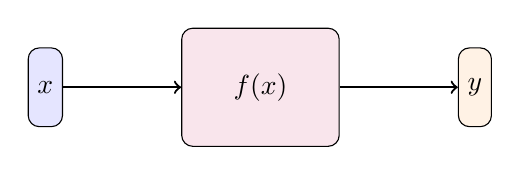
\begin{tikzpicture}
            \node[draw, rounded corners, minimum height=1cm, fill=blue!10] (input) {$x$};
            \node[draw, rounded corners, minimum width=2cm, minimum height=1.5cm, right=1.5cm of input, fill=purple!10] (function) {$f(x)$};
            \node[draw, rounded corners, minimum height=1cm, right=1.5cm of function, fill=orange!10] (output) {$y$};
            
            \draw[->, thick] (input) -- (function);
            \draw[->, thick] (function) -- (output);
        \end{tikzpicture}
    \end{center}
    
    \begin{center}
        \includegraphics[width=0.7\textwidth]{figures/model_diagram.png}
    \end{center}
\end{frame}

\begin{frame}{Exemple avec un LLM}
    \begin{center}
        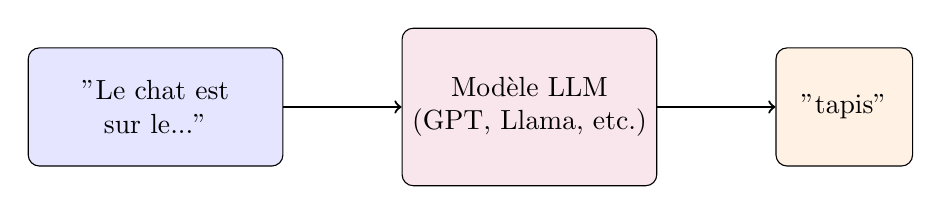
\begin{tikzpicture}
            \node[draw, rounded corners, text width=3cm, minimum height=1.5cm, align=center, fill=blue!10] (input) {"Le chat est sur le..."};
            \node[draw, rounded corners, text width=3cm, minimum height=2cm, right=1.5cm of input, align=center, fill=purple!10] (model) {Modèle LLM\\(GPT, Llama, etc.)};
            \node[draw, rounded corners, text width=1.5cm, minimum height=1.5cm, right=1.5cm of model, align=center, fill=orange!10] (output) {"tapis"};
            
            \draw[->, thick] (input) -- (model);
            \draw[->, thick] (model) -- (output);
        \end{tikzpicture}
    \end{center}
    
    \begin{itemize}
        \item Un \textbf{LLM} (Large Language Model) prend du texte en entrée
        \item Il prédit le mot ou la séquence suivante la plus probable
        \item Ce processus peut être répété pour générer des textes entiers
    \end{itemize}
\end{frame}

\begin{frame}{Génération de texte causale (autoregressive)}
    \begin{center}
        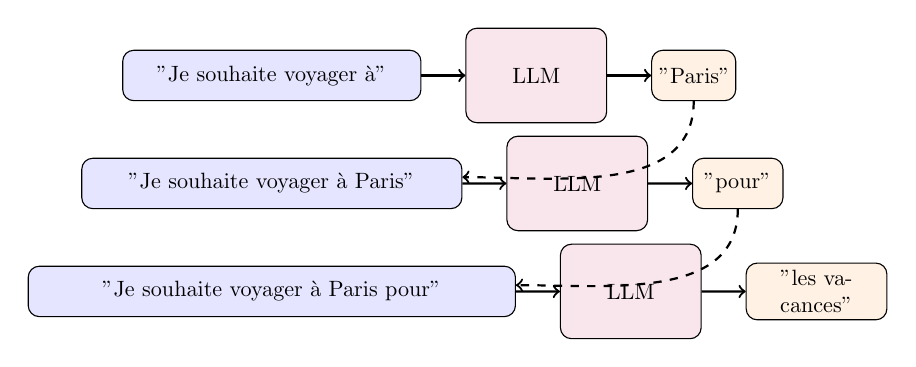
\begin{tikzpicture}[scale=0.8, transform shape, node distance=0.4cm]
            % Étape initiale
            \node[draw, rounded corners, text width=4.5cm, minimum height=0.8cm, align=center, fill=blue!10] (prompt) {"Je souhaite voyager à"};
            \node[draw, rounded corners, text width=2cm, minimum height=1.5cm, right=0.7cm of prompt, align=center, fill=purple!10] (model1) {LLM};
            \node[draw, rounded corners, text width=1.1cm, minimum height=0.8cm, right=0.7cm of model1, align=center, fill=orange!10] (output1) {"Paris"};
            
            % Deuxième étape
            \node[draw, rounded corners, text width=5.8cm, minimum height=0.8cm, align=center, fill=blue!10, below=0.9cm of prompt] (prompt2) {"Je souhaite voyager à Paris"};
            \node[draw, rounded corners, text width=2cm, minimum height=1.5cm, right=0.7cm of prompt2, align=center, fill=purple!10] (model2) {LLM};
            \node[draw, rounded corners, text width=1.2cm, minimum height=0.8cm, right=0.7cm of model2, align=center, fill=orange!10] (output2) {"pour"};
            
            % Troisième étape
            \node[draw, rounded corners, text width=7.5cm, minimum height=0.8cm, align=center, fill=blue!10, below=0.9cm of prompt2] (prompt3) {"Je souhaite voyager à Paris pour"};
            \node[draw, rounded corners, text width=2cm, minimum height=1.5cm, right=0.7cm of prompt3, align=center, fill=purple!10] (model3) {LLM};
            \node[draw, rounded corners, text width=2cm, minimum height=0.8cm, right=0.7cm of model3, align=center, fill=orange!10] (output3) {"les vacances"};
            
            % Flèches
            \draw[->, thick] (prompt) -- (model1);
            \draw[->, thick] (model1) -- (output1);
            \draw[->, thick] (prompt2) -- (model2);
            \draw[->, thick] (model2) -- (output2);
            \draw[->, thick] (prompt3) -- (model3);
            \draw[->, thick] (model3) -- (output3);
            
            % Flèches de continuité entre étapes
            \draw[->, thick, dashed] (output1.south) to[out=-90,in=0] ($(prompt2.east) + (0,0.1)$);
            \draw[->, thick, dashed] (output2.south) to[out=-90,in=0] ($(prompt3.east) + (0,0.1)$);
        \end{tikzpicture}
    \end{center}
    
    \begin{itemize}
        \item \textbf{Génération causale} : prédiction \textbf{mot par mot}
        \item Chaque prédiction est ajoutée au contexte
        \item Le modèle génère le texte de façon \textbf{séquentielle}
        \item Il ne "connaît" pas les mots futurs pendant la génération
    \end{itemize}
\end{frame}

\begin{frame}{L'entraînement des modèles}
    \begin{columns}
        \column{0.4\textwidth}
        \begin{itemize}
            \item Les modèles sont optimisés sur d'énormes volumes de données
            \item L'objectif: ajuster les paramètres internes pour minimiser les erreurs
            \item Pour les LLMs: des milliers de milliards de mots issus d'Internet
        \end{itemize}
        
        \column{0.6\textwidth}
        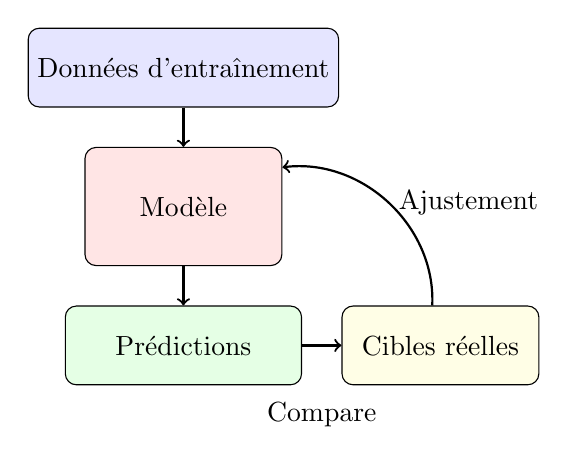
\begin{tikzpicture}
            \node[draw, rounded corners, minimum width=3cm, minimum height=1cm, fill=blue!10] (data) {Données d'entraînement};
            \node[draw, rounded corners, minimum width=2.5cm, minimum height=1.5cm, below=0.5cm of data, fill=red!10] (model) {Modèle};
            \node[draw, rounded corners, minimum width=3cm, minimum height=1cm, below=0.5cm of model, fill=green!10] (output) {Prédictions};
            \node[draw, rounded corners, minimum width=2.5cm, minimum height=1cm, right=0.5cm of output, fill=yellow!10] (target) {Cibles réelles};
            
            \draw[->, thick] (data) -- (model);
            \draw[->, thick] (model) -- (output);
            \draw[->, thick] (output) -- node[below, yshift=-0.6cm] {Compare} (target);
            \draw[->, thick, bend right=50] (target) to node[right] {Ajustement} (model);
        \end{tikzpicture}
    \end{columns}
\end{frame}


\begin{frame}{Points clés à retenir}
    \begin{itemize}
        \item Derrière toute IA générative se trouve un \textbf{modèle}
        \item Ce modèle est entraîné sur une \textbf{énorme base de données} (souvent issue d'Internet)
        \item C'est un modèle \textbf{statistique} qui reproduit les patterns observés
        \item Deux sources d'information limitent le modèle:
            \begin{itemize}
                \item Son \textbf{entraînement} (limité dans le temps)
                \item Sa \textbf{fenêtre de contexte} (la question et les informations fournies)
            \end{itemize}
    \end{itemize}
    
    \begin{center}
        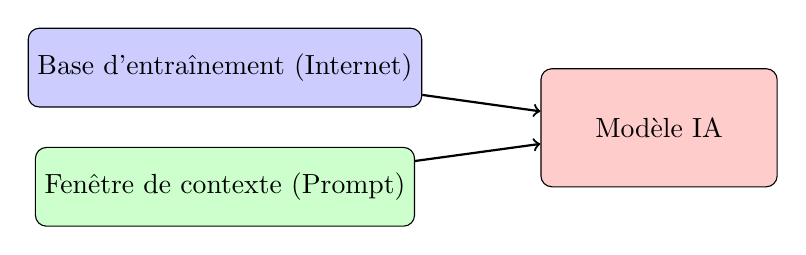
\begin{tikzpicture}
            \node[draw, rounded corners, fill=blue!20, minimum width=4cm, minimum height=1cm] (training) {Base d'entraînement (Internet)};
            \node[draw, rounded corners, fill=green!20, minimum width=4cm, minimum height=1cm, below=0.5cm of training] (context) {Fenêtre de contexte (Prompt)};
            \node[draw, rounded corners, fill=red!20, minimum width=3cm, minimum height=1.5cm, below right=-0.5cm and 1.5cm of training] (model) {Modèle IA};
            
            \draw[->, thick] (training) -- (model);
            \draw[->, thick] (context) -- (model);
        \end{tikzpicture}
    \end{center}
\end{frame}

\end{document}
